\documentclass{article}

% if you need to pass options to natbib, use, e.g.:
% \PassOptionsToPackage{numbers, compress}{natbib}
% before loading nips_2016
%
% to avoid loading the natbib package, add option nonatbib:
% \usepackage[nonatbib]{nips_2016}

%\usepackage{nips_2016}

% to compile a camera-ready version, add the [final] option, e.g.:
% \usepackage[final]{nips_2016}

\usepackage[utf8]{inputenc} % allow utf-8 input
\usepackage[T1]{fontenc}    % use 8-bit T1 fonts
\usepackage[hidelinks]{hyperref}       % hyperlinks
\usepackage{url}            % simple URL typesetting
\usepackage{booktabs}       % professional-quality tables
\usepackage{amsfonts}       % blackboard math symbols
\usepackage{nicefrac}       % compact symbols for 1/2, etc.
\usepackage{cleveref}		
\usepackage{microtype}      % microtypography
\usepackage{listings}
\usepackage{mathtools} 
\usepackage{graphicx}
\usepackage{subcaption}
\usepackage{csvsimple}


\title{An Analysis of Image Denoising Techniques}
\usepackage[final]{nips_2016}

% The \author macro works with any number of authors. There are two
% commands used to separate the names and addresses of multiple
% authors: \And and \AND.
%
% Using \And between authors leaves it to LaTeX to determine where to
% break the lines. Using \AND forces a line break at that point. So,
% if LaTeX puts 3 of 4 authors names on the first line, and the last
% on the second line, try using \AND instead of \And before the third
% author name.

\author{
  Benjamin A. Schifman\\
  Department of Electrical and Computer Engineering\\
  University of Arizona\\
  Tucson, AZ 85719 \\
  \texttt{bschifman@email.arizona.edu} \\
  %% examples of more authors
  %% \And
  %% Coauthor \\
  %% Affiliation \\
  %% Address \\
  %% \texttt{email} \\
  %% \AND
  %% Coauthor \\
  %% Affiliation \\
  %% Address \\
  %% \texttt{email} \\
  %% \And
  %% Coauthor \\
  %% Affiliation \\
  %% Address \\
  %% \texttt{email} \\
  %% \And
  %% Coauthor \\
  %% Affiliation \\
  %% Address \\
  %% \texttt{email} \\
}

\begin{document}
 

\maketitle

\begin{abstract}
  Digital denoising techniques are used to filter out unwanted noise in a signal. In images, noisy signals are present in the form of non coherent Salt \& Pepper noise and Gaussian noise to coherent noise introduced inherently from the imager or from signal processing algorithms. This paper examines some of the common methods for removing unwanted noise, along with implementing more adept filtering techniques in the form wavelet filtering. 
\end{abstract}

\section{Introduction}
 This paper explores noise filtering techniques implemented in Python and an available Python image processing library $OpenCV.$ The filters are implemented on images with random Gaussian noise and Salt \& Pepper noise, and their output Peak Signal to Noise Ratios are compared. The two $python$ files are detailed in section \ref{Software_Lisiting}. The underlying input image $FIGURE X$ and it's corresponding noisy images $Noisy IMAGES$ are in this figure. The standard filters that were implemented using the $OpenCV$ library were the: \textit{blur, gaussian blur, median} and \textit{bilateral} filter and the filter windows were varied in order to generate the optimal resulting filter. The Haar Wavelet Transform was implemented by hand, and the Daubechies 4 wavelet was implemented using the available $PyWavelets$ library after an attempt by hand of the algorithm was unsuccessful.

\section{Methods/Approach}
\subsection{Noise Generation}
Two images were generated with different noise distributions for the purpose of analyzing the efficacy of the different applied filtering techniques. The first noisy image was generated with a normal Gaussian distribution that had been scaled by a factor of $10$. The noise was scaled in order to be more visually evident in the image along with increasing the noise power in the image. Gaussian noise is generally a common form of noise that principally arises in images during acquisition and is caused by a number of factors, a few being poor illumination, high circuitry temperature, and electronic interference. The second noisy image was generated through adding a $0.4\%$ Salt \& Pepper (S\&P) distribution. The S\&P noise added was equally distributed "Salt" white pixels, and "Pepper" black pixels. S\&P noise potentially occurs in images were intermittent and non-reliable image communication systems are present as they can elicit sharp and sudden disturbances in the image signal. The following Figure~\ref{fig:noisy_cman} depicts the noise induced images.

\begin{figure}[h!]
	\centering
	\begin{subfigure}[b]{0.45\linewidth}
		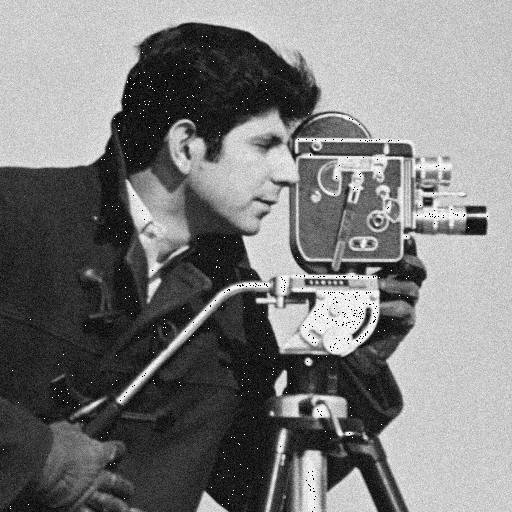
\includegraphics[width=\linewidth]{../../2_Software/data/cman_gnoise.png}
		\caption{cman w\ Gaussian Noise}
	\end{subfigure}
	\begin{subfigure}[b]{0.45\linewidth}
		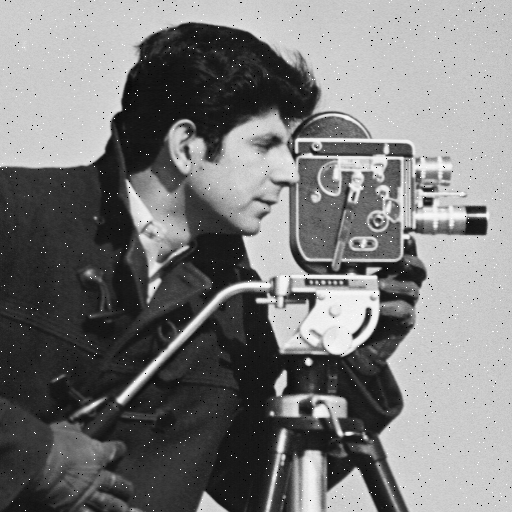
\includegraphics[width=\linewidth]{../../2_Software/data/cman_spnoise.png}
		\caption{cman w\ S\&P Noise}
	\end{subfigure}
	\caption{Noisy cman Images}
	\label{fig:noisy_cman}
\end{figure}

\subsection{Peak Signal to Noise Ratio}
In order to analyze the utility of the aforementioned filtering techniques the Peak Signal to Noise Ratios (PSNR) for each filtered image was calculated. The PSNR of an image is the maximum power of an image and the power of the image noise. The following equation \ref{eqn:PSNR} details the calculations for PSNR.
\begin{equation}\label{eqn:PSNR}
PSNR = 10*log_{10}\Big(\frac{MAX^2}{MSE}\Big)
\end{equation}	 
Where $MAX$ is the maximum grayscale pixel value for the image which in this case is an unsigned 8-bit image with a maximum value of 255, and the $MSE$ is the Mean Squared Error between the filtered output image and the noisy image. By taking the maximum pixel
 
\subsection{Haar Wavelet Transform}
The Haar Wavelet Transform (HWT), proposed by the Hungarian mathematician Alfr\'ed Haar is a computationally efficient method for analyzing the local aspects of an image. A key advantage to the use and implementation of the HWT is in it simplicity to compute, along with it being easier to understand than most other wavelet transforms. A great benefit to using the HWT is that it is effective in signal and image compression and the algorithm is a memory efficient in that all of the calculations can be done in place, however, the software depicted below uses temporary vectors for ease of following. The HWT can be expressed in terms of matrix operations such that the Forward HWT is:  

\begin{equation}\label{eqn:Forward_HWT}
y_{n} = W_{n}v_{n}
\end{equation}	 
 
 where $v_{n}$ is the input vector to be transformed, $W_{n}$ is the HWT matrix, and $y_{n}$ is the transformed output vector. This calculation can be even more easily illustrated in the form of the following expanded graphic in Figure~\ref{fig:Haar_Forward} that details the Haar transform of an input vector of length $8$, its corresponding Haar Matrix $W_{8}$, and its output vector which is simply the mean or trend of two sequential pixel elements for the first half of the vector, and then the second half of the values are a running difference or fluctuation of two sequential pixel elements. 
 
 \begin{figure}[h!]
 	\centering
	\includegraphics[width=\linewidth]{../../1_Resources/images/Haar_matrix_8.png}
	\caption{Haar Transform}
 	\label{fig:Haar_Forward}
 \end{figure}
 
 The algorithm for this vector-wise HWT has been implemented by hand in the software and can be found in the $OneD\textunderscore HWT$ function in the $DWT.py$ file. On a 2D image the HWT is first calculated on the rows of the image, and then the HWT is calculated on the columns of the image. This 2D implementation can be found in the $TwoD\textunderscore HWT$ in the $DWT.py$ file. This 2D function also accounts for multiple iterations of the HWT in that each following iteration will reduce the image into smaller sub-wavelets.  
 The Inverse HWT can be calculated by the following equation with the same variables:
 
 \begin{equation}\label{eqn:Inverse_HWT}
 x_{n} = H^Ty_{n}
 \end{equation}
 
 The HWT can be 
 
\subsection{Daubechies Wavelet Transform}
\subsection{Thresholding}
Pixel thresholding is often a simple but efficient non-linear denoising approach in the application of a wavelet transform. The thresholding is performed on the wavelet transformed image, and then the image is inverse wavelet transformed to yield a filtered output image. To determine the best threshold value to set, the $detThreshold$ function from $dataSetup.py$ was used. This function first iterates through thresholding values, then thresholds the Wavelet Transformed image, then inverse Wavelet Transforms the thresholded image, and finally calculates the Peak Signal to Noise ratio of the filtered image. The threshold is chosen based off of the one that results in the largest Peak Signal to Noise Ratio. The following equations \eqref{eqn:Hard Threshold} and \eqref{eqn:Soft Threshold} detail the Hard and Soft Thresholding calculations respectively, with Figure~\ref{fig:thresholding} depicting the thresholds.
\\\\
Hard Thresholding   
\begin{equation}\label{eqn:Hard Threshold}
D^H(d|T) =
\begin{cases}
0, & \text{if $|d| \leq T$} \\
d, & \text{if $|d| > T$} \\
\end{cases}
\end{equation}	
Soft Thresholding
\begin{equation}\label{eqn:Soft Threshold}
D^S(d|T) =
\begin{cases}
0, & \text{if $|d| \leq T$} \\
d-T, & \text{if $d > T$} \\
d+T, & \text{if $d < -T$}
\end{cases}
\end{equation} 
\begin{figure}[h!]
	\centering
	\begin{subfigure}[b]{0.4\linewidth}
		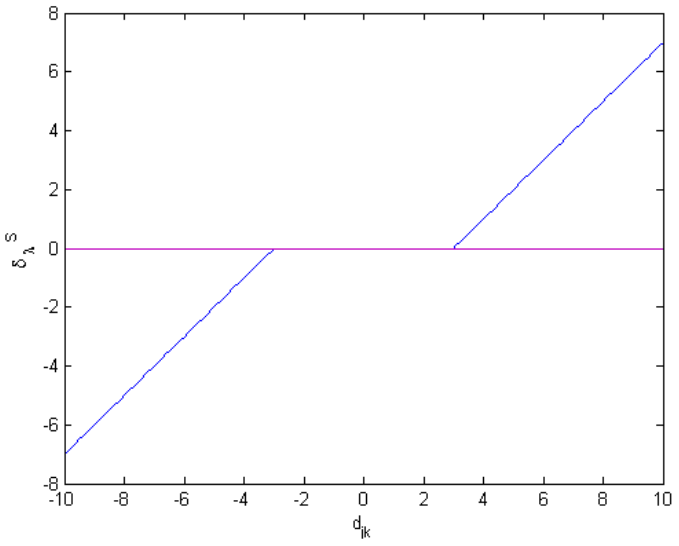
\includegraphics[width=\linewidth]{../../1_Resources/images/hard_thresholding.png}
		\caption{Hard Threshold.}
	\end{subfigure}
	\begin{subfigure}[b]{0.4\linewidth}
		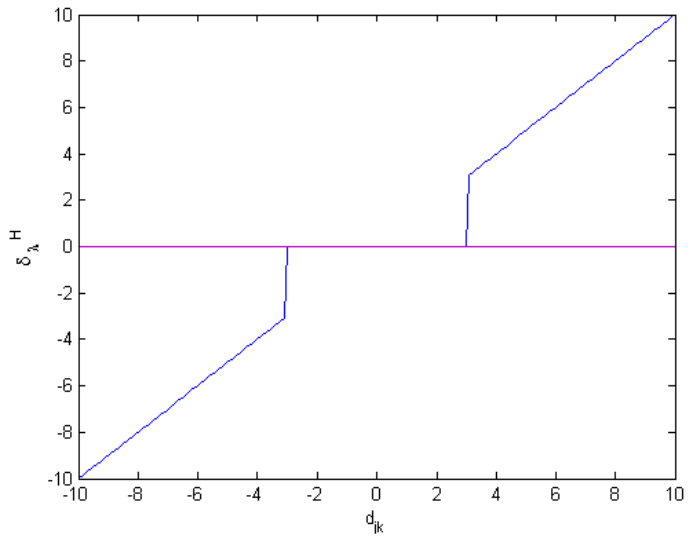
\includegraphics[width=\linewidth]{../../1_Resources/images/soft_thresholding.png}
		\caption{Soft Threshold.}
	\end{subfigure}	
	\caption{Thresholding Methods}
	\label{fig:thresholding}
\end{figure}

The following Figure depicts the PSNR of the filtered wavelet transforms vs. a given threshold value, and the threshold value was chosen that resulted in the greatest PSNR value.

\begin{figure}[h!]
	\centering
	\begin{subfigure}[b]{0.45\linewidth}
		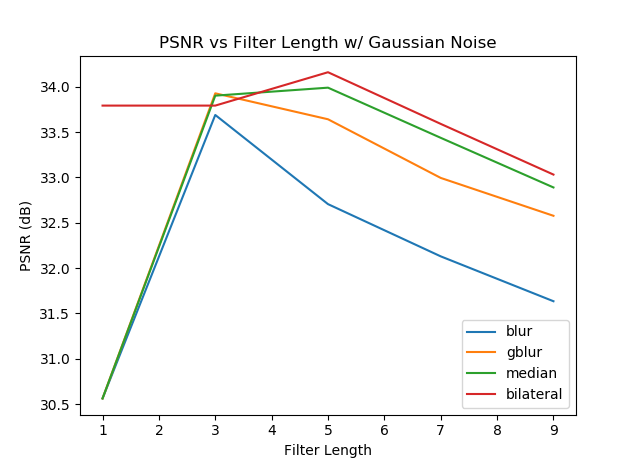
\includegraphics[width=\linewidth]{../../1_Resources/images/filter_length_g.png}
		\caption{Hard Threshold.}
	\end{subfigure}
	\begin{subfigure}[b]{0.45\linewidth}
		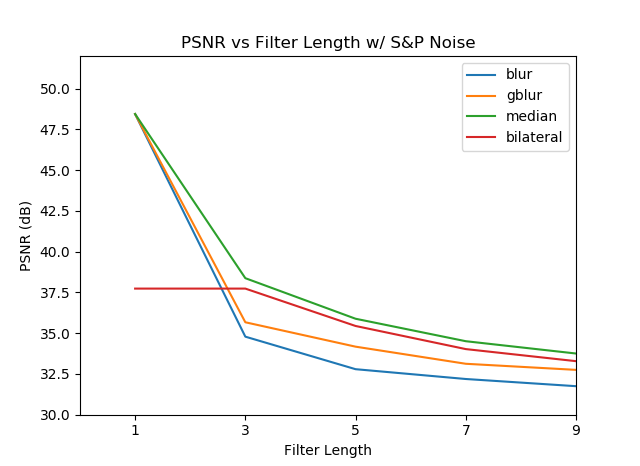
\includegraphics[width=\linewidth]{../../1_Resources/images/filter_length_sp.png}
		\caption{Soft Threshold.}
	\end{subfigure}	
	\caption{PSNR vs. Filter Lengths}
	\label{fig:filter_length}
\end{figure}

\begin{figure}[h!]
	\centering
	\begin{subfigure}[b]{0.45\linewidth}
		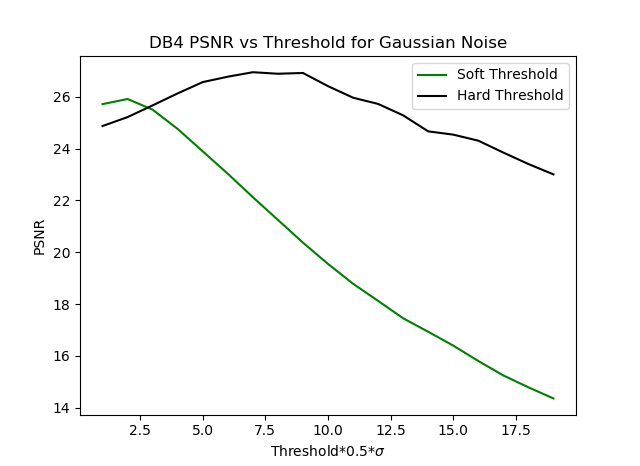
\includegraphics[width=\linewidth]{../../1_Resources/images/DB4_threshold_g.png}
		\caption{DB4 w\ Gaussian Noise}
	\end{subfigure}
	\begin{subfigure}[b]{0.45\linewidth}
		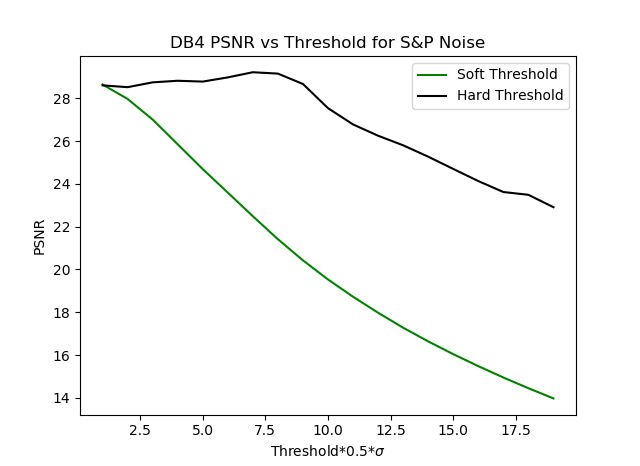
\includegraphics[width=\linewidth]{../../1_Resources/images/DB4_threshold_sp.png}
		\caption{DB4 w\ S\&P Noise}
	\end{subfigure}
	\begin{subfigure}[b]{0.45\linewidth}
		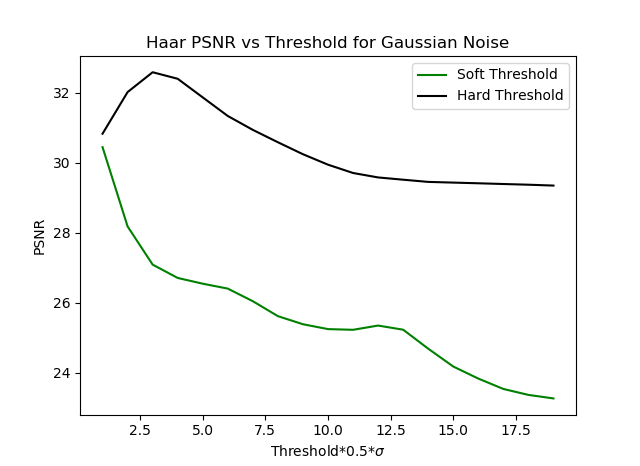
\includegraphics[width=\linewidth]{../../1_Resources/images/HWT_threshold_g.png}
		\caption{HWT w\ Gaussian Noise}
	\end{subfigure}
	\begin{subfigure}[b]{0.45\linewidth}
		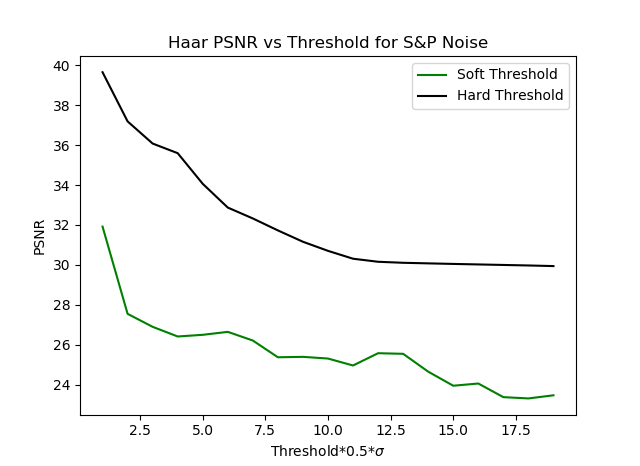
\includegraphics[width=\linewidth]{../../1_Resources/images/HWT_threshold_sp.png}
		\caption{HWT w\ S\&P Noise.}
	\end{subfigure}	
	\caption{PSNR vs. Thresholding Value}
	\label{fig:psnr_threshold}
\end{figure}


\section{Results}
\centering
\csvautotabular{../../2_Software/psnr_final.csv}

\section{Conclusion}


\begin{figure}[h!]
	\centering
	\begin{subfigure}[b]{0.45\linewidth}
		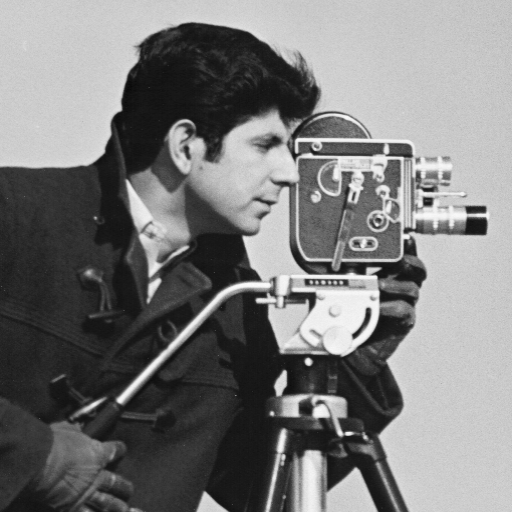
\includegraphics[width=\linewidth]{../../2_Software/data/cman_512_512.png}
		\caption{cman}
	\end{subfigure}
	\begin{subfigure}[b]{0.45\linewidth}
		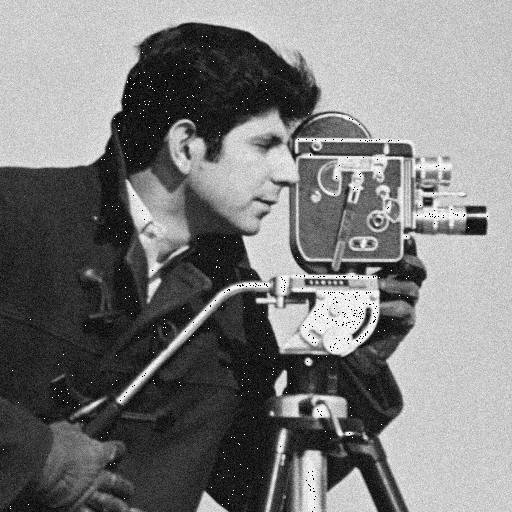
\includegraphics[width=\linewidth]{../../2_Software/data/cman_gnoise.png}
		\caption{cman w\ Gaussian Noise}
	\end{subfigure}
	\begin{subfigure}[b]{0.45\linewidth}
		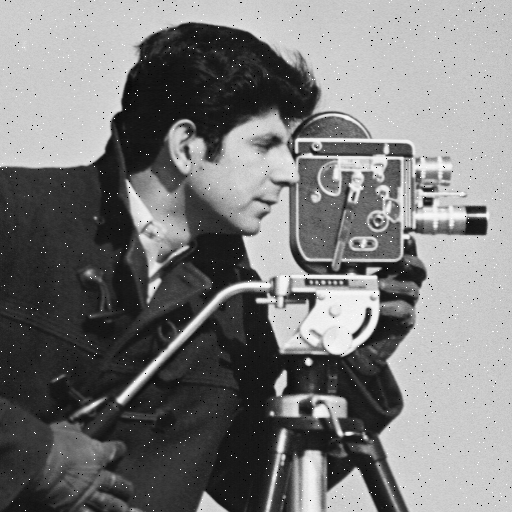
\includegraphics[width=\linewidth]{../../2_Software/data/cman_spnoise.png}
		\caption{cman w\ S\&P Noise}
	\end{subfigure}
	\caption{PSNR vs. Thresholding Value}
	\label{fig:psnr_threshold}
\end{figure}




\section*{References}

References follow the acknowledgments. Use unnumbered first-level
heading for the references. Any choice of citation style is acceptable
as long as you are consistent. It is permissible to reduce the font
size to \verb+small+ (9 point) when listing the references. {\bf
  Remember that you can use a ninth page as long as it contains
  \emph{only} cited references.}
\medskip

\small

[1] Alexander, J.A.\ \& Mozer, M.C.\ (1995) Template-based algorithms
for connectionist rule extraction. In G.\ Tesauro, D.S.\ Touretzky and
T.K.\ Leen (eds.), {\it Advances in Neural Information Processing
  Systems 7}, pp.\ 609--616. Cambridge, MA: MIT Press.

[2] Bower, J.M.\ \& Beeman, D.\ (1995) {\it The Book of GENESIS:
  Exploring Realistic Neural Models with the GEneral NEural SImulation
  System.}  New York: TELOS/Springer--Verlag.

[3] Hasselmo, M.E., Schnell, E.\ \& Barkai, E.\ (1995) Dynamics of
learning and recall at excitatory recurrent synapses and cholinergic
modulation in rat hippocampal region CA3. {\it Journal of
  Neuroscience} {\bf 15}(7):5249-5262.


\section{Software Lisiting}\label{Software_Lisiting}
\subsection{dataSetup}
%\lstinputlisting[language=Python]{../../2_Software/dataSetup.py}
\subsection{DWT}
%\lstinputlisting[language=Python]{../../2_Software/DWT.py}
\end{document}